\section{The Gram-Schmidt orthogonalization procedure}
\label{sec:gram-schmidt}

\begin{outcome}
  \begin{enumerate}
  \item Use the Gram-Schmidt procedure to find an orthogonal basis
    of a subspace of an inner product space.
  \item Find an orthonormal basis of a subspace.
  \end{enumerate}
\end{outcome}

Although we have already seen some potential uses for orthogonal
bases, we have not yet seen very many examples of such bases. In this
section, we will look at the Gram-Schmidt orthogonalization procedure,
a method for turning any basis into an orthogonal one.

The basic idea is very simple: if two vectors $\vect{v}_1,\vect{v}_2$
are not orthogonal, then we can make them orthogonal by replacing
$\vect{v}_2$ by a vector of the form $\vect{u}_2 = \vect{v}_2 -
t\vect{v}_1$, for a suitable parameter $t$.
\begin{equation*}
  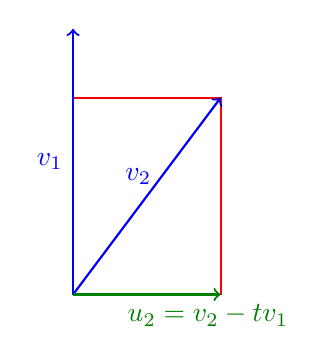
\begin{tikzpicture}[scale=1.25]
    \draw[thick,red] (1.5,0) -- (1.5,2) -- (0,2);
    \draw[thick,blue,->] (0,0) -- node[left]{$\vect{v}_1$} (0,2.7);
    \draw[thick,blue,->] (0,0) -- node[left, pos=0.6]{$\vect{v}_2$} (1.5,2);
    \draw[thick,green!50!black,->] (0,0) -- node[below right, pos=0.3]{$\vect{u}_2 = \vect{v}_2 - t\vect{v}_1$} (1.5,0);
  \end{tikzpicture}
\end{equation*}
But what is the correct value of $t$? It turns out that this value is
uniquely determined by the requirement that $\vect{v}_1$ and
$\vect{u}_2$ must be orthogonal. We calculate
\begin{equation*}
  \iprod{\vect{v}_1,\vect{u}_2}
  ~=~ \iprod{\vect{v}_1,\vect{v}_2-t\vect{v}_1}
  ~=~ \iprod{\vect{v}_1,\vect{v}_2}-t\iprod{\vect{v}_1,\vect{v}_1}.
\end{equation*}
Setting this equal to $0$ yields the unique solution
\begin{equation*}
  t = \frac{\iprod{\vect{v}_1,\vect{v}_2}}{\iprod{\vect{v}_1,\vect{v}_1}}
\end{equation*}
Note that this is exactly the same thing as the Fourier coefficient of
$\vect{v}_2$ in the direction of $\vect{v}_1$. The following
proposition summarizes what we have found so far. For consistency with
our later notation, we also rename the first basis vector $\vect{v}_1$
to $\vect{u}_1$.

\begin{proposition}{Gram-Schmidt orthogonalization procedure for 2 vectors}{gram-schmidt-2}
  Let $\set{\vect{v}_1,\vect{v}_2}$ be a basis for some subspace $W$
  of an inner product space $V$. Define vectors
  $\vect{u}_1,\vect{u}_2$ as follows:
  \begin{eqnarray*}
    \vect{u}_1 &=& \vect{v}_1, \\
    \vect{u}_2 &=& \vect{v}_2 ~-~ \frac{\iprod{\vect{u}_1,\vect{v}_2}}{\iprod{\vect{u}_1,\vect{u}_1}}\vect{u}_1.
  \end{eqnarray*}
  Then $\set{\vect{u}_1,\vect{u}_2}$ is an orthogonal basis of $W$.
\end{proposition}

\begin{example}{Gram-Schmidt orthogonalization procedure for 2 vectors}{gram-schmidt-2}
  In $\R^3$ with the usual dot product, find an orthogonal basis for
  \begin{equation*}
    \sspan\set{
      \begin{mymatrix}{c} 1 \\ 1 \\ 0 \end{mymatrix},~
      \begin{mymatrix}{c} 0 \\ 1 \\ 1 \end{mymatrix}
    }.
  \end{equation*}
\end{example}

\begin{solution}
  Let $\vect{v}_1 = \begin{mymatrix}{c} 1 \\ 1 \\ 0 \end{mymatrix}$
  and $\vect{v}_2 = \begin{mymatrix}{c} 0 \\ 1 \\ 1 \end{mymatrix}$.
  We calculate
  \begin{eqnarray*}
    \vect{u}_1
    &=& \vect{v}_1
        ~=~ \begin{mymatrix}{c} 1 \\ 1 \\ 0 \end{mymatrix}, \\
    \vect{u}_2
    &=& \vect{v}_2 ~-~ \frac{\iprod{\vect{u}_1,\vect{v}_2}}{\iprod{\vect{u}_1,\vect{u}_1}}\vect{u}_1
        ~=~ \begin{mymatrix}{c} 0 \\ 1 \\ 1 \end{mymatrix}
    ~-~ \frac{1}{2}\begin{mymatrix}{c} 1 \\ 1 \\ 0 \end{mymatrix}
    ~=~ \begin{mymatrix}{c} -1/2 \\ 1/2 \\ 1 \end{mymatrix}.
  \end{eqnarray*}
  Therefore the desired orthogonal basis is
  $\set{\begin{mymatrix}{c} 1 \\ 1 \\ 0 \end{mymatrix},
    \begin{mymatrix}{c} -1/2 \\ 1/2 \\ 1 \end{mymatrix}}$.
\end{solution}

The procedure for finding an orthogonal basis of a $k$-dimensional
space is very similar. We adjust each basis vector $\vect{v}_i$ by
subtracting a suitable linear combination of previous orthogonal basis
vectors.

\begin{proposition}{Gram-Schmidt orthogonalization procedure for $k$ vectors}{gram-schmidt-k}
  Let $\set{\vect{v}_1,\ldots,\vect{v}_k}$ be a basis for some subspace $W$
  of an inner product space $V$.%
  \index{Gram-Schmidt procedure}%
  \index{orthogonalization}%
  \index{orthogonal basis!Gram-Schmidt procedure}
  Define vectors
  $\vect{u}_1,\ldots,\vect{u}_k$ as follows:
  \begin{eqnarray*}
    \vect{u}_1
    &=& \vect{v}_1,
    \\
    \vect{u}_2
    &=& \vect{v}_2
        ~-~ \frac{\iprod{\vect{u}_1,\vect{v}_2}}{\iprod{\vect{u}_1,\vect{u}_1}}\vect{u}_1,
    \\
    \vect{u}_3
    &=& \vect{v}_3
        ~-~ \frac{\iprod{\vect{u}_1,\vect{v}_3}}{\iprod{\vect{u}_1,\vect{u}_1}}\vect{u}_1
        ~-~ \frac{\iprod{\vect{u}_2,\vect{v}_3}}{\iprod{\vect{u}_2,\vect{u}_2}}\vect{u}_2,
    \\
    &\vdots&
    \\
    \vect{u}_k
    &=& \vect{v}_k
        ~-~ \frac{\iprod{\vect{u}_1,\vect{v}_k}}{\iprod{\vect{u}_1,\vect{u}_1}}\vect{u}_1
        ~-~ \frac{\iprod{\vect{u}_2,\vect{v}_k}}{\iprod{\vect{u}_2,\vect{u}_2}}\vect{u}_2
        ~-~ \ldots
        ~-~ \frac{\iprod{\vect{u}_{k-1},\vect{v}_k}}{\iprod{\vect{u}_{k-1},\vect{u}_{k-1}}}\vect{u}_{k-1}.
  \end{eqnarray*}
  Then $\set{\vect{u}_1,\ldots,\vect{u}_k}$ is an orthogonal basis of $W$.
\end{proposition}

\begin{proof}
  First, it is clear that $\set{\vect{v}_1,\ldots,\vect{v}_k}$ and
  $\set{\vect{u}_1,\ldots,\vect{u}_k}$ span the same subspace, as each
  $\vect{v}_i$ is a linear combination of
  $\vect{u}_1,\ldots,\vect{u}_i$ and conversely, each $\vect{u}_i$ is
  a linear combination of $\vect{v}_1,\ldots,\vect{v}_i$. So the only
  thing we must check is that $\set{\vect{u}_1,\ldots,\vect{u}_k}$ is
  an orthogonal set. In other words, we must show that
  $\iprod{\vect{u}_j,\vect{u}_i}=0$ for all $j<i$. We prove this by
  induction on $i$, i.e., we assume it is already true for all pairs
  of indices smaller than $i$. To show
  $\iprod{\vect{u}_j,\vect{u}_i}=0$, we calculate:
  \begin{eqnarray*}
    \iprod{\vect{u}_j,\vect{u}_i}
    &=& \textstyle
        \iprod{\vect{u}_j, \vect{v}_i
        ~-~ \frac{\iprod{\vect{u}_1,\vect{v}_i}}{\iprod{\vect{u}_1,\vect{u}_1}}\vect{u}_1
        ~-~ \ldots
        ~-~ \frac{\iprod{\vect{u}_j,\vect{v}_i}}{\iprod{\vect{u}_j,\vect{u}_j}}\vect{u}_j
        ~-~ \ldots
        ~-~ \frac{\iprod{\vect{u}_{i-1},\vect{v}_i}}{\iprod{\vect{u}_{i-1},\vect{u}_{i-1}}}\vect{u}_{i-1}}
    \\
    &=& \textstyle
        \iprod{\vect{u}_j, \vect{v}_i}
        ~-~ \frac{\iprod{\vect{u}_1,\vect{v}_i}}{\iprod{\vect{u}_1,\vect{u}_1}}\iprod{\vect{u}_j,\vect{u}_1}
        ~-~ \ldots
        ~-~ \frac{\iprod{\vect{u}_j,\vect{v}_i}}{\iprod{\vect{u}_j,\vect{u}_j}}\iprod{\vect{u}_j,\vect{u}_j}
        ~-~ \ldots
        ~-~ \frac{\iprod{\vect{u}_{i-1},\vect{v}_i}}{\iprod{\vect{u}_{i-1},\vect{u}_{i-1}}}\iprod{\vect{u}_j,\vect{u}_{i-1}}
    \\
    &=& \textstyle
        \iprod{\vect{u}_j, \vect{v}_i}
        ~-~ 0
        ~-~ \ldots
        ~-~ \frac{\iprod{\vect{u}_j,\vect{v}_i}}{\iprod{\vect{u}_j,\vect{u}_j}}\iprod{\vect{u}_j,\vect{u}_j}
        ~-~ \ldots
        ~-~ 0
    \\
    &=& \iprod{\vect{u}_j, \vect{v}_i}
        ~-~ \iprod{\vect{u}_j,\vect{v}_i}
    \\
    &=& 0.
  \end{eqnarray*}
  It follows that the set $\set{\vect{u}_1,\ldots,\vect{u}_k}$ is
  orthogonal, as desired.
\end{proof}

\begin{example}{Gram-Schmidt orthogonalization procedure}{gram-schmidt-r4}
  In $\R^4$, find an orthogonal basis for
  \begin{equation*}
    \sspan\set{
      \begin{mymatrix}{c} 1 \\ 1 \\ 1 \\ 1 \end{mymatrix},~
      \begin{mymatrix}{c} 1 \\ 1 \\ 1 \\ 0 \end{mymatrix},~
      \begin{mymatrix}{c} 1 \\ 1 \\ 0 \\ 0 \end{mymatrix}
    }.
  \end{equation*}
\end{example}

\begin{solution}
  Let
  \begin{equation*}
    \vect{v}_1 = \begin{mymatrix}{c} 1 \\ 1 \\ 1 \\ 1 \end{mymatrix},\quad
    \vect{v}_2 = \begin{mymatrix}{c} 1 \\ 1 \\ 1 \\ 0 \end{mymatrix},\quad\mbox{and}\quad
    \vect{v}_3 = \begin{mymatrix}{c} 1 \\ 1 \\ 0 \\ 0 \end{mymatrix}.
  \end{equation*}
  We calculate
  \begin{eqnarray*}
    \vect{u}_1
    &=& \vect{v}_1
        ~=~ \begin{mymatrix}{c} 1 \\ 1 \\ 1 \\ 1 \end{mymatrix},
    \\
    \vect{u}_2
    &=& \vect{v}_2 ~-~ \frac{\iprod{\vect{u}_1,\vect{v}_2}}{\iprod{\vect{u}_1,\vect{u}_1}}\vect{u}_1
    ~=~ \begin{mymatrix}{c} 1 \\ 1 \\ 1 \\ 0 \end{mymatrix}
    ~-~ \frac{3}{4}\begin{mymatrix}{c} 1 \\ 1 \\ 1 \\ 1 \end{mymatrix}
    ~=~ \begin{mymatrix}{c} 1/4 \\ 1/4 \\ 1/4 \\ -3/4 \end{mymatrix},
    \\
    \vect{u}_3
    &=& \vect{v}_3
        ~-~ \frac{\iprod{\vect{u}_1,\vect{v}_3}}{\iprod{\vect{u}_1,\vect{u}_1}}\vect{u}_1
        ~-~ \frac{\iprod{\vect{u}_2,\vect{v}_3}}{\iprod{\vect{u}_2,\vect{u}_2}}\vect{u}_2
    \\
    &=& \begin{mymatrix}{c} 1 \\ 1 \\ 0 \\ 0 \end{mymatrix}
    ~-~ \frac{2}{4}\begin{mymatrix}{c} 1 \\ 1 \\ 1 \\ 1 \end{mymatrix}
    ~-~ \frac{1/2}{3/4}\begin{mymatrix}{c} 1/4 \\ 1/4 \\ 1/4 \\ -3/4 \end{mymatrix}
    ~=~ \begin{mymatrix}{c} 1/3 \\ 1/3 \\ -2/3 \\ 0 \end{mymatrix}.
  \end{eqnarray*}
  Therefore the orthogonal basis is
  $\set{\vect{u}_1,\vect{u}_2,\vect{u}_3} = \set{
    \begin{mymatrix}{c} 1 \\ 1 \\ 1 \\ 1 \end{mymatrix},~
    \begin{mymatrix}{c} 1/4 \\ 1/4 \\ 1/4 \\ -3/4 \end{mymatrix},~
    \begin{mymatrix}{c} 1/3 \\ 1/3 \\ -2/3 \\ 0 \end{mymatrix}
  }$.
\end{solution}

The Gram-Schmidt procedure is sensitive to reordering the vectors. For
example, if we order the original basis vectors in
Example~\ref{exa:gram-schmidt-r4} in the opposite order, we end up
with a different orthogonal basis at the end. Sometimes this can
simplify the calculations, as the following example shows.

\begin{example}{Gram-Schmidt orthogonalization procedure: reordering the vectors}{gram-schmidt-r4-b}
  In $\R^4$, find an orthogonal basis for
  \begin{equation*}
    \sspan\set{
      \begin{mymatrix}{c} 1 \\ 1 \\ 0 \\ 0 \end{mymatrix},~
      \begin{mymatrix}{c} 1 \\ 1 \\ 1 \\ 0 \end{mymatrix},~
      \begin{mymatrix}{c} 1 \\ 1 \\ 1 \\ 1 \end{mymatrix}
    }.
  \end{equation*}
\end{example}

\begin{solution}
  Note that these are the same basis vectors as in
  Example~\ref{exa:gram-schmidt-r4}, but listed in a different order.
  Let
  \begin{equation*}
    \vect{v}_1 = \begin{mymatrix}{c} 1 \\ 1 \\ 0 \\ 0 \end{mymatrix},\quad
    \vect{v}_2 = \begin{mymatrix}{c} 1 \\ 1 \\ 1 \\ 0 \end{mymatrix},\quad\mbox{and}\quad
    \vect{v}_3 = \begin{mymatrix}{c} 1 \\ 1 \\ 1 \\ 1 \end{mymatrix}.
  \end{equation*}
  We calculate
  \begin{eqnarray*}
    \vect{u}_1
    &=& \vect{v}_1
        ~=~ \begin{mymatrix}{c} 1 \\ 1 \\ 0 \\ 0 \end{mymatrix},
    \\
    \vect{u}_2
    &=& \vect{v}_2 ~-~ \frac{\iprod{\vect{u}_1,\vect{v}_2}}{\iprod{\vect{u}_1,\vect{u}_1}}\vect{u}_1
    ~=~ \begin{mymatrix}{c} 1 \\ 1 \\ 1 \\ 0 \end{mymatrix}
    ~-~ \frac{2}{2}\begin{mymatrix}{c} 1 \\ 1 \\ 0 \\ 0 \end{mymatrix}
    ~=~ \begin{mymatrix}{c} 0 \\ 0 \\ 1 \\ 0 \end{mymatrix},
    \\
    \vect{u}_3
    &=& \vect{v}_3
        ~-~ \frac{\iprod{\vect{u}_1,\vect{v}_3}}{\iprod{\vect{u}_1,\vect{u}_1}}\vect{u}_1
        ~-~ \frac{\iprod{\vect{u}_2,\vect{v}_3}}{\iprod{\vect{u}_2,\vect{u}_2}}\vect{u}_2
    \\
    &=& \begin{mymatrix}{c} 1 \\ 1 \\ 1 \\ 1 \end{mymatrix}
    ~-~ \frac{2}{2}\begin{mymatrix}{c} 1 \\ 1 \\ 0 \\ 0 \end{mymatrix}
    ~-~ \frac{1}{1}\begin{mymatrix}{c} 0 \\ 0 \\ 1 \\ 0 \end{mymatrix}
    ~=~ \begin{mymatrix}{c} 0 \\ 0 \\ 0 \\ 1 \end{mymatrix}.
  \end{eqnarray*}
  This time, we end up with the orthogonal basis
  $\set{\vect{u}_1,\vect{u}_2,\vect{u}_3} = \set{
    \begin{mymatrix}{c} 1 \\ 1 \\ 0 \\ 0 \end{mymatrix},~
    \begin{mymatrix}{c} 0 \\ 0 \\ 1 \\ 0 \end{mymatrix},~
    \begin{mymatrix}{c} 0 \\ 0 \\ 0 \\ 1 \end{mymatrix}
  }$.
\end{solution}

In the next example, we will consider $\R^n$, but with a non-standard
inner product.

\begin{example}{Gram-Schmidt orthogonalization procedure, non-standard inner product}{gram-schmidt-non-standard}
  Let
  \begin{equation*}
    A = \begin{mymatrix}{ccc}
      1 & 2 & -2 \\
      2 & 6 & -1 \\
      -2 & -1 & 9 \\
    \end{mymatrix},
  \end{equation*}
  and consider the vector space $\R^3$ with the inner product given by
  $\iprod{\vect{v},\vect{w}} = \vect{v}^T A\vect{w}$.
  Let
  \begin{equation*}
    \vect{v}_1 = \begin{mymatrix}{c} 1 \\ 0 \\ 0 \end{mymatrix},
    \quad
    \vect{v}_2 = \begin{mymatrix}{c} 0 \\ 1 \\ 0 \end{mymatrix},
    \quad\mbox{and}\quad
    \vect{v}_3 = \begin{mymatrix}{c} 0 \\ 0 \\ 1 \end{mymatrix}.
  \end{equation*}
  Apply the Gram-Schmidt procedure to
  $\vect{v}_1,\vect{v}_2,\vect{v}_3$ to find an orthogonal basis
  $\set{\vect{u}_1,\vect{u}_2,\vect{u}_3}$ for $\R^3$ with respect to
  the above inner product.
\end{example}

\begin{solution}
  As usual, we start with
  \begin{eqnarray*}
    \vect{u}_1 &=& \vect{v}_1 = \begin{mymatrix}{c} 1 \\ 0 \\ 0 \end{mymatrix}.
  \end{eqnarray*}
  Next, we calculate
  \begin{eqnarray*}
    \iprod{\vect{u}_1,\vect{v}_2} &=& \vect{u}_1^TA\vect{v}_2 = 2, \\
    \iprod{\vect{u}_1,\vect{u}_1} &=& \vect{u}_1^TA\vect{u}_1 = 1.
  \end{eqnarray*}
  Therefore,
  \begin{eqnarray*}
    \vect{u}_2
    &=& \vect{v}_2
        - \frac{\iprod{\vect{u}_1,\vect{v}_2}}{\iprod{\vect{u}_1,\vect{u}_1}} \vect{u}_1
        = \begin{mymatrix}{c} 0 \\ 1 \\ 0 \end{mymatrix}
    - \frac{2}{1} \begin{mymatrix}{c} 1 \\ 0 \\ 0 \end{mymatrix}
    = \begin{mymatrix}{c} -2 \\ 1 \\ 0 \end{mymatrix}.
  \end{eqnarray*}
  Finally, we calculate
  \begin{eqnarray*}
    \iprod{\vect{u}_1,\vect{v}_3} &=& \vect{u}_1^TA\vect{v}_3 = -2, \\
    \iprod{\vect{u}_2,\vect{v}_3} &=& \vect{u}_2^TA\vect{v}_3 = 3, \\
    \iprod{\vect{u}_2,\vect{u}_2} &=& \vect{u}_2^TA\vect{u}_2 = 2.
  \end{eqnarray*}
  Therefore,
  \begin{eqnarray*}
    \vect{u}_3
    &=& \vect{v}_3
        - \frac{\iprod{\vect{u}_1,\vect{v}_3}}{\iprod{\vect{u}_1,\vect{u}_1}} \vect{u}_1
        - \frac{\iprod{\vect{u}_2,\vect{v}_3}}{\iprod{\vect{u}_2,\vect{u}_2}} \vect{u}_2
        = \begin{mymatrix}{c} 0 \\ 0 \\ 1 \end{mymatrix}
    - \frac{-2}{1} \begin{mymatrix}{c} 1 \\ 0 \\ 0 \end{mymatrix}
    - \frac{3}{2} \begin{mymatrix}{c} -2 \\ 1 \\ 0 \end{mymatrix}
    = \begin{mymatrix}{c} 5 \\ -3/2 \\ 1 \end{mymatrix}.
  \end{eqnarray*}
  So the desired orthogonal basis is
  \begin{equation*}
    \set{\vect{u}_1,\vect{u}_2,\vect{u}_3}
    = \set{
      \begin{mymatrix}{c} 1 \\ 0 \\ 0 \end{mymatrix},
      \begin{mymatrix}{c} -2 \\ 1 \\ 0 \end{mymatrix},
      \begin{mymatrix}{c} 5 \\ -3/2 \\ 1 \end{mymatrix}
    }.
  \end{equation*}
  Note that it is not orthogonal with respect to the dot product, but
  with respect to the inner product defined above.
\end{solution}

\begin{example}{Legendre polynomials}{legendre-polynomials}
  Consider the vector space $\Poly$ of polynomials, with the inner product
  \begin{equation*}
    \iprod{p,q} = \int_{-1}^{1} p(x)q(x)\,dx.
  \end{equation*}
  Use the Gram-Schmidt procedure to find an orthogonal basis for
  $\sspan\set{1,x,x^2,x^3}$.%
  \index{Legendre polynomial}%
  \index{polynomial!Legendre polynomial}
\end{example}

\begin{solution}
  Let $\vect{v}_1=1$, $\vect{v}_2=x$, $\vect{v}_3=x^2$, and
  $\vect{v}_4=x^3$. We follow the Gram-Schmidt procedure:
  \begin{eqnarray*}
    \vect{u}_1
    &=& \vect{v}_1
        ~=~ 1.
  \end{eqnarray*}
  Before we calculate $\vect{u}_2$, we have to evaluate two integrals:
  \begin{eqnarray*}
    \iprod{\vect{u}_1,\vect{v}_2}
    &=& \int_{-1}^{1} 1\cdot x\,dx
    ~=~ \bigbracket{\textstyle\frac{1}{2}x^2}_{-1}^{1}
    ~=~ 0,
    \\
    \iprod{\vect{u}_1,\vect{u}_1}
    &=& \int_{-1}^{1} 1\cdot 1\,dx
    ~=~ \bigbracket{x}_{-1}^{1}
    ~=~ 2.
  \end{eqnarray*}
  Then
  \begin{eqnarray*}
    \vect{u}_2
    &=& \vect{v}_2 ~-~ \frac{\iprod{\vect{u}_1,\vect{v}_2}}{\iprod{\vect{u}_1,\vect{u}_1}}\vect{u}_1
    ~=~ x ~-~ \frac{0}{2}\cdot 1 ~=~ x.
  \end{eqnarray*}
  To calculate $\vect{u}_3$, we first evaluate three integrals:
  \begin{eqnarray*}
    \iprod{\vect{u}_1,\vect{v}_3}
    &=& \int_{-1}^{1} 1\cdot x^2\,dx
    ~=~ \bigbracket{\textstyle\frac{1}{3}x^3}_{-1}^{1}
    ~=~ \frac{2}{3},
    \\
    \iprod{\vect{u}_2,\vect{v}_3}
    &=& \int_{-1}^{1} x\cdot x^2\,dx
    ~=~ \bigbracket{\textstyle\frac{1}{4}x^4}_{-1}^{1}
    ~=~ 0,
    \\
    \iprod{\vect{u}_2,\vect{u}_2}
    &=& \int_{-1}^{1} x\cdot x\,dx
    ~=~ \bigbracket{\textstyle\frac{1}{3}x^3}_{-1}^{1}
    ~=~ \frac{2}{3}.
  \end{eqnarray*}
  Then
  \begin{eqnarray*}
    \vect{u}_3
    &=& \vect{v}_3
        ~-~ \frac{\iprod{\vect{u}_1,\vect{v}_3}}{\iprod{\vect{u}_1,\vect{u}_1}}\vect{u}_1
        ~-~ \frac{\iprod{\vect{u}_2,\vect{v}_3}}{\iprod{\vect{u}_2,\vect{u}_2}}\vect{u}_2
        ~=~ x^2 ~-~ \frac{2/3}{2}\cdot 1 ~-~ \frac{0}{2/3}\cdot x
        ~=~ x^2 - \frac{1}{3}.
  \end{eqnarray*}
  To calculate $\vect{u}_4$, we first evaluate four integrals:
  \begin{eqnarray*}
    \iprod{\vect{u}_1,\vect{v}_4}
    &=& \int_{-1}^{1} 1\cdot x^3\,dx
    ~=~ \bigbracket{\textstyle\frac{1}{4}x^4}_{-1}^{1}
    ~=~ 0,
    \\
    \iprod{\vect{u}_2,\vect{v}_4}
    &=& \int_{-1}^{1} x\cdot x^3\,dx
    ~=~ \bigbracket{\textstyle\frac{1}{5}x^5}_{-1}^{1}
    ~=~ \frac{2}{5},
    \\
    \iprod{\vect{u}_3,\vect{v}_4}
    &=& \int_{-1}^{1}\textstyle (x^2-\frac{1}{3})\cdot x^3\,dx
    ~=~ \bigbracket{\textstyle\frac{1}{6}x^6 - \frac{1}{12}x^4}_{-1}^{1}
    ~=~ 0,
    \\
    \iprod{\vect{u}_3,\vect{u}_3}
    &=& \int_{-1}^{1}\textstyle (x^2-\frac{1}{3})^2\,dx
    ~=~ \bigbracket{\textstyle\frac{1}{5}x^5-\frac{2}{9}x^3+\frac{1}{9}x}_{-1}^{1}
    ~=~ \frac{8}{45}.
  \end{eqnarray*}
  Then
  \begin{eqnarray*}
    \vect{u}_4
    &=& \vect{v}_4
        ~-~ \frac{\iprod{\vect{u}_1,\vect{v}_4}}{\iprod{\vect{u}_1,\vect{u}_1}}\vect{u}_1
        ~-~ \frac{\iprod{\vect{u}_2,\vect{v}_4}}{\iprod{\vect{u}_2,\vect{u}_2}}\vect{u}_2
        ~-~ \frac{\iprod{\vect{u}_3,\vect{v}_4}}{\iprod{\vect{u}_3,\vect{u}_3}}\vect{u}_3
    \\
    &=& x^3 ~-~ \frac{0}{2}\cdot 1 ~-~ \frac{2/5}{2/3}\cdot x ~-~ \frac{0}{8/45}\cdot(x^2-\frac{1}{3})
        ~=~ x^3 - \frac{3}{5}x.
  \end{eqnarray*}
  Thus, we obtain the orthogonal basis $\set{\vect{u}_1,\vect{u}_2,\vect{u}_3,\vect{u}_4} =
  \set{1,~ x,~ x^2-\frac{1}{3},~ x^3 - \frac{3}{5}x}$.
\end{solution}

The orthogonal polynomials from Example~\ref{exa:legendre-polynomials}
are known (up to scalar multiples) as \textbf{Legendre polynomials}%
\index{Legendre polynomial}%
\index{polynomial!Legendre polynomial}.  We can continue in the same
fashion applying the Gram-Schmidt procedure to the polynomials
$1, x, x^2, x^3, x^4, x^5, x^6, \ldots$ to get an infinite sequence of
orthogonal polynomials. The first few elements of this sequence are:
\begin{eqnarray*}
  p_0(x) &=& 1, \\
  p_1(x) &=& x, \\
  p_2(x) &=& x^2 - \frac{1}{3}, \\
  p_3(x) &=& x^3 - \frac{3}{5}x, \\
  p_4(x) &=& x^4 - \frac{6}{7}x^2 + \frac{3}{35}, \\
  p_5(x) &=& x^5 - \frac{10}{9}x^3 + \frac{5}{21}x, \\
  p_6(x) &=& x^6 - \frac{15}{11}x^4 + \frac{5}{11}x^2 - \frac{5}{231}, \\
  p_7(x) &=& x^7 - \frac{21}{13}x^5 + \frac{105}{143}x^3 - \frac{35}{429}x, \\
  p_8(x) &=& x^8 - \frac{28}{15}x^6 + \frac{14}{13}x^4 - \frac{28}{143}x^2 + \frac{7}{1287}.
\end{eqnarray*}
\begin{center}
  \begin{tikzpicture}[domain=1:-1, scale=4]
    \draw[thick,color=fourier1,samples=50] plot (\x,{abs(\x^6)-15/11*abs(\x^4)+5/11*abs(\x^2)-5/231}) node[left=2ex,color=fourier1t] {$x^6 - \frac{15}{11}x^4 + \frac{5}{11}x^2 - \frac{5}{231}$};
    \draw[thick,color=fourier2,samples=50] plot (\x,{\x^5 - 10/9*\x^3+5/21*\x}) node[left=2ex,color=fourier2t] {$x^5 - \frac{10}{9}x^3 + \frac{5}{21}x$};
    \draw[thick,color=fourier3,samples=50] plot (\x,{abs(\x^4)-6/7*abs(\x^2)+3/35}) node[left=2ex,color=fourier3t] {$x^4 - \frac{6}{7}x^2 + \frac{3}{35}$};
    \draw[thick,color=fourier4,samples=50] plot (\x,\x^3-3/5*\x) node[left=2ex,color=fourier4t] {$x^3 - \frac{3}{5}x$};
    \draw[thick,color=fourier5,samples=50] plot (\x,{abs(\x^2)-1/3}) node[left=2ex,,color=fourier5t] {$x^2-\frac{1}{3}$};
    \draw[thick,color=fourier6] plot (\x,\x) node[left=2ex,color=fourier6t] {$x$};
    \draw[thick,color=fourier7] plot (\x,1) node[left=2ex,color=fourier7t] {$1$};
    \draw[->] (-1.2,0) -- (1.2,0) node[right] {$x$};
    \draw[->] (0,-1.2) -- (0,1.2) node[above] {$p(x)$};
    \draw (1,0) -- (1,-0.05) node[below] {$1$};
    \draw (-1,0) -- (-1,-0.05) node[below] {$-1$};
  \end{tikzpicture}
\end{center}

The Gram-Schmidt procedure yields an {\em orthogonal} basis. If we
want to compute an {\em orthonormal} basis, we also have to normalize
each basis vector. Since normalization usually involves dividing by a
square root, it is best to do this at the end, i.e., after the entire
Gram-Schmidt procedure is complete, rather than normalizing each
$\vect{u}_i$ immediately after it is found. Note that the Gram-Schmidt
procedure itself does not involve computing any square roots.

\begin{example}{Finding an orthonormal basis}{finding-orthonormal-basis-r4}
  In $\R^4$, find an orthogonal basis for
  \begin{equation*}
    \sspan\set{
      \begin{mymatrix}{c} 1 \\ 1 \\ 1 \\ 1 \end{mymatrix},~
      \begin{mymatrix}{c} 1 \\ 1 \\ 1 \\ 0 \end{mymatrix},~
      \begin{mymatrix}{c} 1 \\ 1 \\ 0 \\ 0 \end{mymatrix}
    }.
  \end{equation*}
\end{example}

\begin{solution}
  In Example~\ref{exa:gram-schmidt-r4}, we already found an orthogonal basis
  \begin{equation*}
    \set{\vect{u}_1,\vect{u}_2,\vect{u}_3} ~=~
    \set{
      \begin{mymatrix}{c} 1 \\ 1 \\ 1 \\ 1 \end{mymatrix},~
      \begin{mymatrix}{c} 1/4 \\ 1/4 \\ 1/4 \\ -3/4 \end{mymatrix},~
      \begin{mymatrix}{c} 1/3 \\ 1/3 \\ -2/3 \\ 0 \end{mymatrix}
    }
  \end{equation*}
  for this space. So all that is left to do is to normalize each
  vector. The orthonormal basis is
  \begin{equation*}
    \set{
      \frac{\vect{u}_1}{\norm{\vect{u}_1}},
      \frac{\vect{u}_2}{\norm{\vect{u}_2}},
      \frac{\vect{u}_3}{\norm{\vect{u}_3}}
    }
    ~=~
    \set{
      \frac{1}{2}\begin{mymatrix}{c} 1 \\ 1 \\ 1 \\ 1 \end{mymatrix},~
      \frac{2}{\sqrt{3}}\begin{mymatrix}{c} 1/4 \\ 1/4 \\ 1/4 \\ -3/4 \end{mymatrix},~
      \frac{\sqrt{3}}{\sqrt{2}}\begin{mymatrix}{c} 1/3 \\ 1/3 \\ -2/3 \\ 0 \end{mymatrix}
    }.
  \end{equation*}
  Alternatively, we could have also normalized the orthogonal basis we
  found in Example~\ref{exa:gram-schmidt-r4-b}. In that case, we
  obtain the orthonormal basis
  \begin{equation*}
    \set{
      \frac{1}{\sqrt{2}}
      \begin{mymatrix}{c} 1 \\ 1 \\ 0 \\ 0 \end{mymatrix},~
      \begin{mymatrix}{c} 0 \\ 0 \\ 1 \\ 0 \end{mymatrix},~
      \begin{mymatrix}{c} 0 \\ 0 \\ 0 \\ 1 \end{mymatrix}
    }.
  \end{equation*}
\end{solution}

\begin{example}{Orthonormal basis of polynomials}{legendre-polynomials2}
  Find an orthonormal basis for the space of
  Example~\ref{exa:legendre-polynomials}.
\end{example}

\begin{solution}
  In Example~\ref{exa:legendre-polynomials}, we found the orthogonal
  basis
  $\set{\vect{u}_1,\vect{u}_2,\vect{u}_3,\vect{u}_4} = \set{1,~ x,~
    x^2-\frac{1}{3},~ x^3 - \frac{3}{5}x}$.  We also computed
  \begin{equation*}
    \iprod{\vect{u}_1,\vect{u}_1} = 2,\quad
    \iprod{\vect{u}_2,\vect{u}_2} = \frac{2}{3},\quad\mbox{and}\quad
    \iprod{\vect{u}_3,\vect{u}_3} = \frac{8}{45}.
  \end{equation*}
  We also need to compute $\iprod{\vect{u}_4,\vect{u}_4}$:
  \begin{equation*}
    \iprod{\vect{u}_4,\vect{u}_4}
    ~=~ \int_{-1}^{1}{\textstyle (x^3 - \frac{3}{5}x)^2}\,dx
    ~=~ \int_{-1}^{1}{\textstyle x^6 - \frac{6}{5}x^4 + \frac{9}{25}x^2}\,dx
    ~=~ \bigbracket{\textstyle\frac{1}{7}x^7-\frac{6}{25}x^5+\frac{3}{25}x^3}_{-1}^{1}
    ~=~ \frac{8}{175}.
  \end{equation*}
  Therefore, the orthonormal basis is:
  \begin{equation*}
    \set{
      \frac{\vect{u}_1}{\norm{\vect{u}_1}},
      \frac{\vect{u}_2}{\norm{\vect{u}_2}},
      \frac{\vect{u}_3}{\norm{\vect{u}_3}},
      \frac{\vect{u}_4}{\norm{\vect{u}_4}}
    }
    = \set{
      \frac{1}{\sqrt{2}},~
      \sqrt{\frac{3}{2}} x,~
      \sqrt{\frac{45}{8}} (x^2-\frac{1}{3}),~
      \sqrt{\frac{175}{8}} (x^3 - \frac{3}{5}x)
    }.
  \end{equation*}
\end{solution}

We finish this section by remarking that the formula
\begin{equation*}
  \frac{\iprod{\vect{u},\vect{v}}}{\iprod{\vect{u},\vect{u}}}\vect{u}
\end{equation*}
is exactly what we called the \textbf{projection of $\vect{v}$ onto
  $\vect{u}$}%
\index{vector!projection of}%
\index{projection!in inner product space}%
\index{projection!vector to vector} in Section~\ref{ssec:projections},
except that we have generalized this concept from $\R^n$ to an
arbitrary inner product space. We can define
\begin{equation*}
  \proj_{\vect{u}}(\vect{v})
  = \frac{\iprod{\vect{u},\vect{v}}}{\iprod{\vect{u},\vect{u}}}\vect{u}.
\end{equation*}
With this definition, the Gram-Schmidt procedure can also be expressed
more succinctly as follows.
\begin{equation*}
  \begin{array}{rcl}
    \vect{u}_1
    &=& \vect{v}_1,
    \\
    \vect{u}_2
    &=& \vect{v}_2
        ~-~ \proj_{\vect{u}_1}(\vect{v}_2),
    \\
    \vect{u}_3
    &=& \vect{v}_3
        ~-~ \proj_{\vect{u}_1}(\vect{v}_3)
        ~-~ \proj_{\vect{u}_2}(\vect{v}_3),
    \\
    &\vdots&
    \\
    \vect{u}_k
    &=& \vect{v}_k
        ~-~ \proj_{\vect{u}_1}(\vect{v}_k)
        ~-~ \proj_{\vect{u}_2}(\vect{v}_k)
        ~-~ \ldots
        ~-~ \proj_{\vect{u}_{k-1}}(\vect{v}_k).
  \end{array}
\end{equation*}

